
\documentclass{beamer}
\usetheme{Pittsburgh}
\usecolortheme{spruce}

% for themes, etc.
\mode<presentation>
{ \usetheme{boxes} }

\usepackage{times}  % fonts are up to you
\usepackage{graphicx}
\usepackage{algorithm}
\usepackage{algorithmic}
\renewcommand{\algorithmicrequire}{\alert{Input:}}
\renewcommand{\algorithmicensure}{\alert{Output:}}

\setbeamertemplate{footline}[frame number]

% these will be used later in the title page
\title{Modular Multiplication \& Application}
\author{Lucas Zewen Ye \\ lucas.zw.ye@outlook.com }
\date{\today}
\url{https://www.bilibili.com/video/BV1yi4y1973u}

\AtBeginSection[]
{
\begin{frame}<beamer> 
\frametitle{Outline} % make a frame titled "Outline"
\setcounter{page}{0}	%setcounter似乎对beamer无效
\tableofcontents[currentsection]  % show TOC and highlight current section
\end{frame}
}


\begin{document}
% this prints title, author etc. info from above
\maketitle

\section{Finite Field}
\begin{frame}{Finite Field}
	A finite field is a finite set that multiplication, addition, subtraction and division (excluding division by zero) are defined and satisfy the rules of arithmetic.

	Given a \alert{prime} $p$, the finite field $GF(p)$ is made up of $0, 1, 2, ..., p-1$ (totally $p$ numbers).

\end{frame}

\section{Modular Operations}
\begin{frame}{Modular Reduction}
	For any integer $a$, it can be written as:

	$a = kp + r$ ($k,p,r$ are all integer, $r < p$ and $k \geq 0$)

	so, $a \bmod p = r$

	\hspace*{\fill}

	Example:

	$20 \bmod 7$, $20 = 2 * 7 + 6$, so $20 \bmod 7 = 6$

	$72 \bmod 13$, $72 = 5 * 13 + 7$, so $72 \bmod 13 = 7$

\end{frame}

\begin{frame}{Operations in Finite Field}
	For any $a, b \in GF(p)$,

	Addition: $(a + b) \bmod p$

	Subtraction: $(a - b) \bmod p$

	Multiplication: $(a  b) \bmod p$

	Inversion: $(inv(a) \cdot a) \bmod p = 1$

	Division: $a / b = (a \cdot inv(b)) \bmod p$
\end{frame}

\begin{frame}{Operations in Finite Field}
	Example: for $p=13, a=7, b=4$

	$a + b = 11$

	$a - b = (7 - 4) \bmod 13 = 3$

	$a * b = 7 * 4 \bmod 13 = 2$

	$inv(b) = 10$

	$a / b = 7 * 10 \bmod 13 = 5$
\end{frame}

\begin{frame}{Properties of Modular Operations}
	$(a + b) \bmod p = (a \bmod p + b \bmod p) \bmod p$

	$(a - b) \bmod p = (a \bmod p - b \bmod p) \bmod p$

	$(a  b) \bmod p = (a \bmod p)   (b \bmod p) \bmod p$

	$((a + b) \bmod p + c) \bmod p = (a + (b + c) \bmod p) \bmod p$

	$((a  b) \bmod p)  c \bmod p = (a  (b  c \bmod p)) \bmod p$

	$((a +b) \bmod p \cdot c) \bmod p = ((a  c) \bmod p + (b  c) \bmod p) \bmod p $
\end{frame}

\begin{frame}{Properties of Modular Operations}
	\alert{Congruences}

	if $a \equiv b \pmod p$, then for any $c, (a + c) \equiv (b + c) \pmod p$

	if $a \equiv b \pmod p$, then for any $c, (a  c) \equiv (b  c) \pmod p$

	if $a \equiv b \pmod p$ and $c \equiv d \pmod p$, then
	\begin{itemize}
		\item	$(a + c) \equiv (b + d) \pmod p$
		\item	$(a - c) \equiv (b - d) \pmod p$
		\item   $(a  c) \equiv (b  d) \pmod p$
		\item   $(a / c) \equiv (b / d) \pmod p$
	\end{itemize}

	\begin{table}[]
		\begin{tabular}{|l|l|l|l|l|}
			\hline
			0  & 1  & 2  & 3  & 4  \\ \hline
			5  & 6  & 7  & 8  & 9  \\ \hline
			10 & 11 & 12 & 13 & 14 \\ \hline
			15 & 16 & 17 & 18 & 19 \\ \hline
		\end{tabular}
	\end{table}
\end{frame}

\section{Modular Algorithms}
\begin{frame}{Basic Modular Reduction}
	1. Use \alert{division}

	$a = kp + r$ ($k,p,r$ are all integer, $r < p$ and $k \geq 0$)

	$k = \lfloor \frac{a}{p} \rfloor$

	$r = a - kp$

	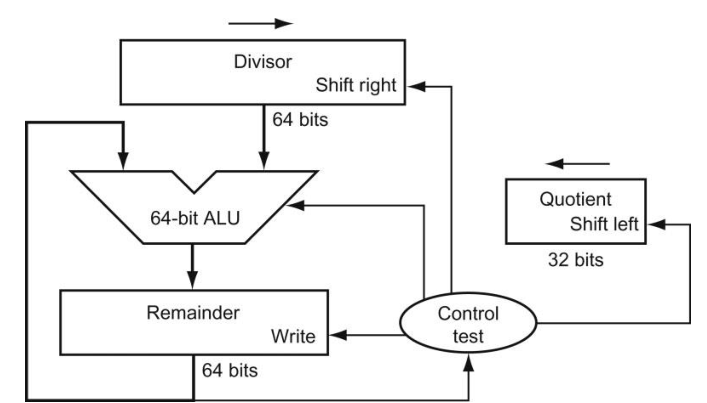
\includegraphics[width=4in]{fig/division.png}

	\centering \alert{\url{http://pages.hmc.edu/harris/research/srtlong.pdf}}
\end{frame}

\begin{frame}{Basic Modular Reduction}
	2. Use \alert{subtractions}

	$a \bmod p = a - p - ... - p$ until the subtraction result is \alert{smaller} than p
\end{frame}

\begin{frame}{Barrett Modular Multiplication}
	Basic idea:

	$a \bmod p = a - \lfloor \frac{a}{p} \rfloor p$, use shift and multiplication to \alert{replcae} the division.

	\hspace*{\fill}

	$t$ is the length of $a$, assume $\frac{1}{p} = \frac{m}{2^t}$, so $m = \frac{2^t}{p}$

	$a \bmod p = a - \lfloor \frac{a*m}{2^t} \rfloor p$
\end{frame}

\begin{frame}{Barrett Modular Multiplication}
	\begin{algorithmic}
		\REQUIRE{$x = (x_{k-1}...x_1x_0)_2$,
			$y = (y_{k-1}...y_1y_0)_2$,
			$p = (p_{k-1}...p_1p_0)_2$,
			$m = \lfloor 2^{2k}/p\rfloor$}
		\ENSURE{$r=xy \ mod \ p$}

		\STATE $z \leftarrow x \cdot y$

		\STATE $q_1 \leftarrow z >> (k-1)$

		\STATE $q_2 \leftarrow q_1 \cdot m$

		\STATE $q_3 \leftarrow q_2 >> (k+1)$

		\STATE $r \leftarrow z - q_3 \cdot p$

		\IF{$r >= 2p$}
		\STATE $r \leftarrow r - 2p$
		\ELSIF{$r >= p$}
		\STATE$r \leftarrow r - p$
		\ENDIF
		\RETURN{$r$}
	\end{algorithmic}
	\alert{Menezes, Alfred J., Paul C. Van Oorschot, and Scott A. Vanstone. Handbook of applied cryptography. CRC press, 2018.}
\end{frame}

\begin{frame}{Montgomery Modular Multiplication}
	$Mont(A,B) = A \cdot B \cdot R^{-1} \bmod N$

	$R$ is the length of $N$, $RR^{-1} \bmod N = 1, RR^{-1} - NN' = 1$


	\begin{itemize}
		\item $T = A \cdot B$
		\item $m =  T \cdot N' \bmod R$
		\item $t = (T + N\cdot m)/R$
		\item $if \ t>N \ return \ (t-N)\  else \  return \ t$
	\end{itemize}

	Prof: Assume $k$ is an integer, and $k < 0$, $m = TN'+kR < R$
	\begin{equation}\nonumber
		\begin{aligned}
			t & = (T + N\cdot m)/R            \\
			  & = (T + N\cdot(TN'+kR)) / R    \\
			  & = (T + TNN' + kRN)/R          \\
			  & = (T(1+NN')+kRN)/R            \\
			  & = TR' + kN                    \\
			  & = A \cdot B \cdot R^{-1} + kN
		\end{aligned}
	\end{equation}

	\alert{Montgomery, Peter L. "Modular multiplication without trial division." Mathematics of computation 44.170 (1985): 519-521.}
\end{frame}

\begin{frame}{Montgomery Modular Multiplication: Multiprecision}
	The large hardware overhead of multiplier:


	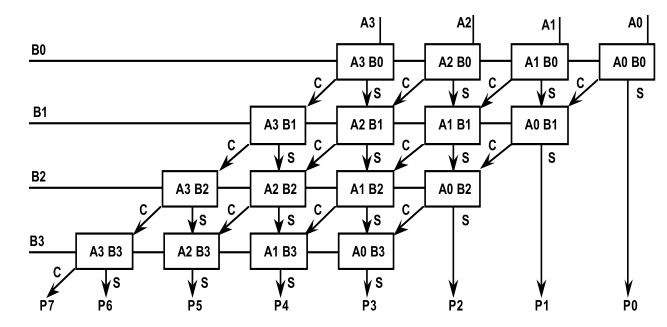
\includegraphics[width=4.3in]{fig/mul.png}
\end{frame}

\begin{frame}{Montgomery Modular Multiplication: Multiprecision}
	789098 × 123456 ÷ 1000000
	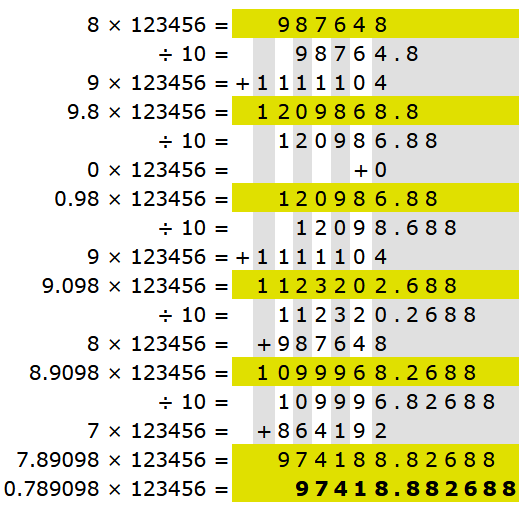
\includegraphics[width=3in]{fig/mont1.png}
\end{frame}

\begin{frame}{Montgomery Modular Multiplication: Multiprecision}
	789098 × 123456 ÷ 1000000 modulo 876543
	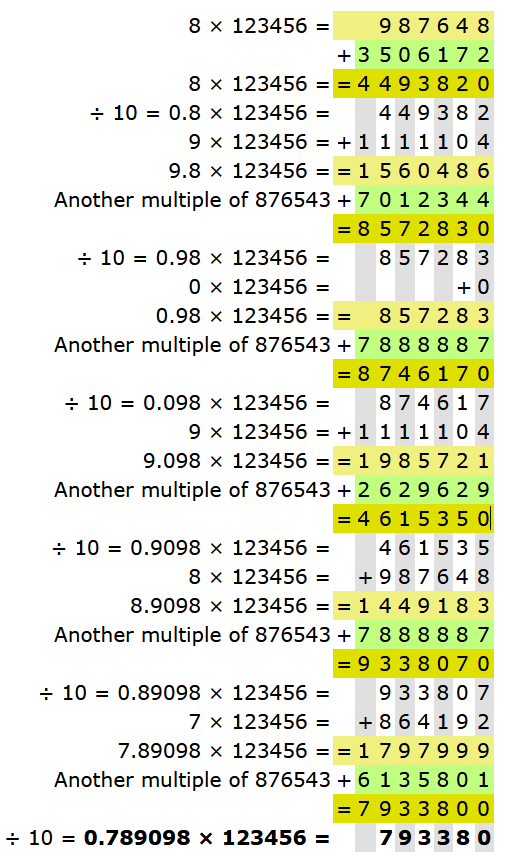
\includegraphics[width=3in]{fig/mont2.png}
\end{frame}

\begin{frame}{Montgomery Modular Multiplication: Multiprecision}
	\begin{algorithmic}
		\REQUIRE{integers $N = (N_{n-1}...N_1N_0)_b$,
		$A = (A_{n-1}...A_1A_0)_b$,
		$B = (B_{n-1}...B_1B_0)_b$ with $0 \leq A, B < N$,
		$R = b^n=(10...0)_b$ with $gcd(N, b) = 1$,
		and $N' = -N^{-1} \bmod b$}
		\ENSURE{$ABR^{-1} \bmod N$}

		\STATE $T \gets 0$

		\FOR{$i \gets 0$ step $1$ to $n-1$}
		\STATE $u_i \gets (T_0 + A_iB_0)N' \bmod b$
		\STATE $T \gets (T+A_iB+u_iN)/b$
		\ENDFOR
		\IF {$T \geq N$}
		\RETURN $T-N$
		\ELSE
		\RETURN $T$
		\ENDIF
	\end{algorithmic}
\end{frame}

\begin{frame}{Montgomery Modular Multiplication: Multiprecision for Hardware}
	\begin{algorithmic}
		\REQUIRE{integers $p = (p_{n-1}...p_1p_0)_2$,
		$A = (A_{n-1}...A_1A_0)_2$,
		$B = (B_{n-1}...B_1B_0)_2$ with $0 \leq A, B < p$,
		$R = 2^n =(10...0)_2$ with $gcd(p, 2) = 1$,
		and $p' = -p^{-1} \bmod 2$}
		\ENSURE{$ABR^{-1} \bmod p$}

		\STATE $T \gets 0$

		\FOR{$i \gets 0$ step $1$ to $n-1$}
		\STATE $u_i \gets (T_0 + A_iB_0)p' \bmod 2$
		\STATE $T \gets (T+A_iB+u_i p)/2$
		\ENDFOR
		\IF {$T \geq p$}
		\RETURN $T-p$
		\ELSE
		\RETURN $T$
		\ENDIF
	\end{algorithmic}
\end{frame}

\section{Application}
\begin{frame}{RSA}
	\begin{table}[]
		\begin{tabular}{|l|l|}
			\hline
			Security Level & Key Size(bit) \\ \hline
			80             & 1024          \\ \hline
			112            & 2048          \\ \hline
			128            & 3072          \\ \hline
			192            & 7680          \\ \hline
			256            & 15360         \\ \hline
		\end{tabular}
	\end{table}
	Given two numbers $p, q$ that satisfy $gcd(p, q) = 1$,
	\begin{itemize}
		\item $n = p\cdot q, L = lcm(p-1, q-1)$
		\item $1 < e < L$ and $gcd(e, L) = 1$
		\item $1 < d < L$ and $e \cdot d \bmod L = 1$
	\end{itemize}
	secret key $(d,n)$, public key $(e,n)$, plaintxt $m$ and ciphertxt $c$

	\begin{itemize}
		\item Encryption: $c = m^e \bmod n$
		\item Decryption: $m = c^d \bmod n$
	\end{itemize}
\end{frame}

\begin{frame}{Post-Quantum Cryptography}
	Given two polynomials $A(x) = \sum_{i=0}^{n-1} a_ix^i$ and $B(x) = \sum_{i=0}^{n-1} b_ix^i \in GF(p^n)$ i.e. $a_i, b_i \in GF(p)$ and the irreducible polynomial $m(x)$

	For \alert{polynomial multiplication}:
	$C(x) = A(x) * B(x) \bmod m(x)= \sum_{i=0}^{2n-2}c_i x^i \bmod m(x), c_i = \sum_{j=0}^{i} a_j b_{i-j} \bmod p$
\end{frame}

\begin{frame}{}
	\centering \Large
	\emph{Thanks}
\end{frame}

\end{document}
